%%%%%%%%%%%%%%%%%%%%%%%%%%%%%%%%%%%%%%%%%%%%%%%%%%%%%%%%%%%%%%%%%%%%%%%%%%%

\documentclass[a4paper,oneside,12pt]{article}
\usepackage{mystyle}

\begin{document}

\title{\Large\bf Exponential functions}
\author{%%
  Minh Van Nguyen \\
  \url{mvngu@gmx.com}
}
\date{\today}
\maketitle


%%%%%%%%%%%%%%%%%%%%%%%%%%%%%%%%%%%%%%%%%%%%%%%%%%%%%%%%%%%%%%%%%%%%%%%%%%%

\section{Growth and decay}

Exponential functions are commonly used to understand the change in a
population over time.  The population can be the residents of a
country, the ants in an ant colony, the bacteria in a Petri dish, or
the amount of carbon-14 in a dinosaur bone.  In particular, what you
want to know is the \emph{percentage rate} of change over time, where
time can be measured in terms of seconds, minutes, hours, days,
months, or years.  If you know the \emph{initial population} and the
percentage rate of change, then you can use the exponential function
to calculate the population in the next year or the next three years.
The following example should help you to understand the ideas
presented above.

\begin{example}
\label{eg:Australian_population_2017}
\textbf{Population of Australia.}
According to the Australian Bureau of Statistics~(ABS), at the end of
September 2017 the population of Australia grew by $1.6\%$ since the
previous year.\footnote{
  ``3101.0 - Australian Demographic Statistics, Sep 2017'',
  \url{http://web.archive.org/web/20180420062713/http://www.abs.gov.au/AUSSTATS/abs@.nsf/Lookup/3101.0Main+Features1Sep\%202017},
  accessed 2018-04-20.
}
The population by the end of the given period was estimated to be
$24.7029$ million people.  Assume that for the next few years the
population of Australia will grow by a rate of $1.6\%$ per annum.
%%
\begin{packedenum}
\item\label{subeg:Australian_population_2017_growth_rate}
  Identify the rate of change.

\item\label{subeg:Australian_population_2017_initial_population}
  Determine the initial population.

\item\label{subeg:Australian_population_2017_table_graph}
  Provide a table of values for the projected population of Australia
  from 2017 to 2021, inclusive.  Graph the data in the table as a
  scatter plot.
\end{packedenum}
\end{example}

\begin{solution}
\solutionpart{subeg:Australian_population_2017_growth_rate}
By the end of September 2017, the population of Australia grew by
$1.6\%$ from the previous year so the percentage rate of change is
$1.6\%$.  Since you are concerned with population growth, the rate of
change in this example is also called the \emph{growth rate}.  The
growth rate can be written as a percentage or as a fraction.  To
express the percentage of $1.6\%$ as a fraction, you divide the number
$1.6$ by $100$ to get the decimal representation
\[
\frac{1.6}{100}
=
0.016.
\]
That is, you can also say that the growth rate is $0.016$.

\solutionpart{subeg:Australian_population_2017_initial_population}
The example does not explicitly state the value of the initial
population.  However, the example does say that the population of
Australia by the end of September 2017 was $24.7029$ million people so
you can consider this number as the initial population.  The reason
why you require an initial population is so that the population can
grow or decline.  You need to start somewhere.

\solutionpart{subeg:Australian_population_2017_table_graph}
You are required to predict the population of Australia from $2018$ to
$2021$, inclusive.  To calculate the projected~(or predicted)
population in $2018$, you must know two numbers: the population in
$2017$ and the growth rate.
From \Part{subeg:Australian_population_2017_growth_rate} you know that
the growth rate is $0.016$ per annum and
from \Part{subeg:Australian_population_2017_initial_population} you
know that the population of Australia for 2017 was $24.7029$ million
people.  By $2018$, the population would have increased by
%%
\begin{equation}
\label{eqn:Australian_population_2018}
24.7029 \times 0.016
=
0.3952464
\end{equation}
%%
million people.  To calculate the population for $2018$, you must add
the number in~\eqref{eqn:Australian_population_2018} to the population
in $2017$.  The projected population for $2018$ is given by the
expression $24.7029 + 24.7029 \times 0.016$.  Factoring out the number
$24.7029$ and simplifying shows that the required population number is
%%
\begin{equation}
\label{eqn:Australian_population_2018_calculation}
\begin{aligned}
24.7029 + 24.7029 \times 0.016
&=
24.7029 (1 + 0.016) \\[4pt]
&=
24.7029 \times 1.016 \\[4pt]
&=
25.0981464
\end{aligned}
\end{equation}
%%
million people.

Now use the same technique as explained above to calculate the
projected population for $2019$.  You already know that the growth
rate is $0.016$ per annum and that the population in $2018$ would be
$25.0981464$ million people.  By $2019$, the population would have
increased by
%%
\begin{equation}
\label{eqn:Australian_population_2019}
25.0981464 \times 0.016
=
0.4015703424
\end{equation}
%%
million people.  The projected population for $2019$ is the number
in~\eqref{eqn:Australian_population_2019} added to the population in
$2018$.  By $2019$ Australia is projected to have a population of
%%
\begin{align*}
25.0981464 + 25.0981464 \times 0.016
&=
25.0981464 (1 + 0.016) \\[4pt]
&=
25.0981464 \times 1.016 \\[4pt]
&=
25.4997167424
\end{align*}
%%
million people.  Use the same technique as explained above to
calculate the projected population in $2020$ and $2021$.  The
projected populations through to the year $2021$ are shown in
\Table{tab:Australian_population_2017}, a graph of which is
illustrated in \Figure{fig:Australian_population_2017}.
\end{solution}

\begin{table}[!htbp]
\centering
\begin{tabular}{cl}           \toprule
Year   & Population         \\\midrule
$2017$ & $24.7029$          \\[4pt]
$2018$ & $25.0981464$       \\[4pt]
$2019$ & $25.4997167424$    \\[4pt]
$2020$ & $25.9077122102784$ \\[4pt]
$2021$ & $26.3222356056429$ \\\bottomrule
\end{tabular}

\caption{%%
  The projected population of Australia through to the year $2021$.
  The population numbers are in terms of millions.  For example, the
  population in $2017$ was estimated to be $24.7029$ million people.
  The population is assumed to grow at a rate of $1.6\%$ per annum.
}
\label{tab:Australian_population_2017}
\end{table}

\begin{figure}[!htbp]
\centering
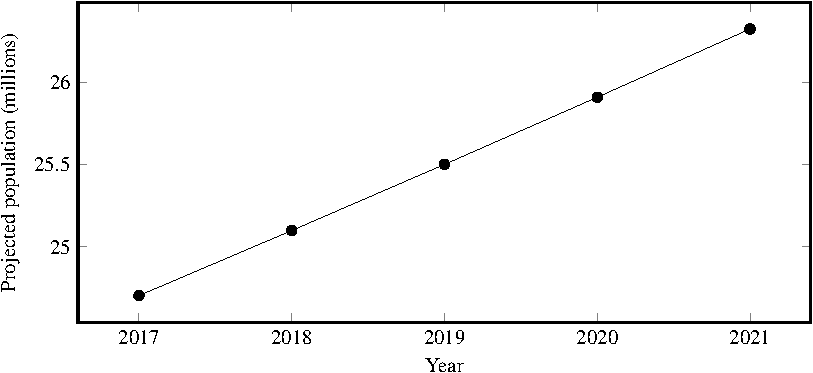
\includegraphics[scale=1]{image/11/australian-population.pdf}
\caption{%%
  The projected population~(in millions) of Australia through to the
  year $2021$.  The population is assumed to grow at a rate of $1.6\%$
  per annum.  Data are from \Table{tab:Australian_population_2017}.
}
\label{fig:Australian_population_2017}
\end{figure}

The next question you might ask is:  Is there a formula to calculate
the population of Australia for any number of years since $2017$?  The
answer is yes, but you must assume that the population grows by a
constant percentage rate each year.  Assume that you have an initial
population of $24.7029$ million people in $2017$ and that the growth
rate is $1.6\%$ or $0.016$ per annum.  According to
\Equation{eqn:Australian_population_2018_calculation}, in
$2018$~(i.e.~one year from $2017$) the population can be written as
the expression
\[
24.7029 + 24.7029 \times 0.016
=
24.7029 \times 1.016.
\]
In $2019$~(i.e.~two years from $2017$) the population can be written
as
%%
\begin{align*}
&24.7029 \times 1.016 + 24.7029 \times 1.016 \times 0.016 \\[4pt]
&=
24.7029 \times 1.016 (1 + 0.016) \\[4pt]
&=
24.7029 \times 1.016 \times 1.016 \\[4pt]
&=
24.7029 \times 1.016^2.
\end{align*}
%%
In $2020$~(i.e.~three years from $2017$) the population can be written
as
%%
\begin{align*}
&24.7029 \times 1.016^2 + 24.7029 \times 1.016^2 \times 0.016 \\[4pt]
&=
24.7029 \times 1.016^2 (1 + 0.016) \\[4pt]
&=
24.7029 \times 1.016^2 \times 1.016 \\[4pt]
&=
24.7029 \times 1.016^3.
\end{align*}
%%
In $2021$~(i.e.~four years from $2017$) the population can be written
as
%%
\begin{align*}
&24.7029 \times 1.016^3 + 24.7029 \times 1.016^3 \times 0.016 \\[4pt]
&=
24.7029 \times 1.016^3 (1 + 0.016) \\[4pt]
&=
24.7029 \times 1.016^3 \times 1.016 \\[4pt]
&=
24.7029 \times 1.016^4.
\end{align*}
%%
From the above equations, you can see that the only number that
changes is the exponent or power of $1.016$.  If $t$ is the number of
years since $2017$, then the population in $t$ years can be written as
%%
\begin{equation}
\label{eqn:Australian_population_formula}
24.7029 \times 1.016^t.
\end{equation}
%%
You can see from \Expression{eqn:Australian_population_formula} that
the initial population is $24.7029$ million people.  The number
$1.016$ is called the \emph{growth factor} and can be written in terms
of the growth rate as $1.016 = 1 + 0.016$.

\begin{exercise}
Use \Expression{eqn:Australian_population_formula} to verify the
population numbers in \Table{tab:Australian_population_2017}.
\end{exercise}

\ifbool{showSolution}{
\begin{solution}
In \Table{tab:Australian_population_2017}, the year $2017$ is $t = 0$
years since $2017$ so according to
\Expression{eqn:Australian_population_formula} the population in
$2017$ is
\[
24.7029 \times 1.016^0
=
24.7029
\]
million people.  The year $2018$ is $t = 1$ year since $2017$ so the
population in $2018$ is
\[
24.7029 \times 1.016^1
=
25.0981464
\]
million people.  The year $2019$ is $t = 2$ years since $2017$ so the
population in $2019$ is
\[
24.7029 \times 1.016^2
=
25.4997167424
\]
million people.  The year $2020$ is $t = 3$ years since $2017$ so the
population in $2020$ is approximately
\[
24.7029 \times 1.016^3
=
25.9077122102784
\]
million people.  Finally, the year $2021$ is $t = 4$ years since
$2017$ so the population in $2021$ is approximately
\[
24.7029 \times 1.016^4
=
26.3222356056429
\]
million people.
\end{solution}
}{}

Let's derive a general formula to model situations such as those
presented in \Example{eg:Australian_population_2017}.  Denote by $a$
the initial value of the population and assume that $a \neq 0$.  Let
$r$ be the decimal representation of the percentage rate of change and
define the growth factor by $b = 1 + r$.  For example, if the
population grows by a constant percentage of $2.3\%$, the decimal
representation of this percentage rate of change is
$r = 2.3 / 100 = 0.023$ and the growth factor is
$b = 1 + 0.023 = 1.023$.  The amount of time since the initial
population is represented by $t$.  So you assume that $t \geq 0$ and
at time $t = 0$ you have the initial population of $a$.  At time
$t = 1$, the population would have changed by an amount of $ar$ since
time $t = 0$.  You add this number to the population at time $t = 0$
to get the population at $t = 1$.  Then the population at time $t = 1$
is given by
\[
a + ar
=
a(1 + r)
=
ab.
\]
At time $t = 2$, the population would have changed by an amount of
$abr$ since time $t = 1$.  You add this number to the population at
time $t = 1$ to get the population at time $t = 2$.  That is, the
population at time $t = 2$ is given by
\[
ab + abr
=
ab(1 + r)
=
abb
=
ab^2.
\]
Now you use the same technique as explained above to obtain the
population at time $t = 3$.  At time $t = 3$, the population would
have changed by an amount of $ab^2r$ since time $t = 2$.  Adding this
number to the population at time $t = 2$ shows that the population at
time $t = 3$ is given by
\[
ab^2 + ab^2r
=
ab^2 (1 + r)
=
ab^2b
=
ab^3.
\]
Use the same technique as explained above to see that the population
at time $t = 4$ is given by the expression
\[
ab^3 + ab^3r
=
ab^3 (1 + r)
=
ab^3b
=
ab^4.
\]
From the above equations, you see that in general the population
$Q(t)$ at time $t \geq 0$ is given by the formula
%%
\begin{align*}
Q(t)
&=
a(1 + r)^t \\[4pt]
&=
ab^t.
\end{align*}
The above discussion is summarised in the next theorem.

\begin{theorem}
\label{thm:exponential_growth}
\textbf{Exponential growth.}
Let $a \neq 0$ be the initial value of a population and assume that
the population changes by a constant decimal rate of $r$ per unit
time.  If $b = 1 + r$ is the growth factor and $Q(t)$ represents the
population number at time $t$, then $Q(t) = ab^t$.
\end{theorem}

\begin{example}
\textbf{Bacterial growth.}
A Petri dish initially contains ten cells of a type of bacteria.  The
bacteria population is known to have a constant percentage growth rate
of $56\%$ per hour.
%%
\begin{packedenum}
\item\label{subeg:bacteria_growth_rate}
  Determine the growth rate and growth factor of the bacteria
  population.

\item\label{subeg:bacteria_initial_population}
  Determine the initial population of bacteria in the Petri dish.

\item\label{subeg:bacteria_growth_1_2_hours}
  Use the same technique as in
  \Expression{eqn:Australian_population_2018_calculation} to calculate
  the number of bacteria in the Petri dish after one hour.  How many
  bacteria would there be in the Petri dish after two hours?

\item\label{subeg:bacteria_growth_formula}
  Derive a formula for the number of bacteria in the Petri dish after
  $t$ hours.  Use the formula to verify your results
  from \Part{subeg:bacteria_growth_1_2_hours}.  Produce a graph of the
  growth of the bacteria population within $24$ hours.
\end{packedenum}
\end{example}

\begin{solution}
\solutionpart{subeg:bacteria_growth_rate}
Since the bacteria population grows at a constant percentage rate of
$56\%$ per hour, the growth rate is $r = 56 / 100 = 0.56$ per hour and
hence the growth factor is $b = 1 + 0.56 = 1.56$.

\solutionpart{subeg:bacteria_initial_population}
The initial population of bacteria is $a = 10$ cells.

\solutionpart{subeg:bacteria_growth_1_2_hours}
You have an initial bacteria population of $10$ cells.  At time
$t = 1$ hour, the bacteria population would have increased by
$10 \times 0.56$ cells.  Add this number to the initial population to
see that after one hour the bacteria population would be
%%
\begin{align*}
10 + 10 \times 0.56
&=
10 (1 + 0.56) \\[4pt]
&=
10 \times 1.56 \\[4pt]
&=
15.6
\end{align*}
%%
cells.  After two hours, the bacteria population would have increased
by $15.6 \times 0.56$ cells.  Adding this number to the population at
time $t = 1$ hour and you have
%%
\begin{align*}
15.6 + 15.6 \times 0.56
&=
15.6 (1 + 0.56) \\[4pt]
&=
15.6 \times 1.56 \\[4pt]
&=
24.336
\end{align*}
%%
cells at time $t = 2$ hours.

\solutionpart{subeg:bacteria_growth_formula}
From \Parts{subeg:bacteria_growth_rate}{subeg:bacteria_initial_population},
you know the initial population to be $a = 10$ cells and the growth
factor is $b = 1.56$.  If $Q(t)$ represents the number of bacteria
cells in the Petri dish after $t$ hours, then use
\Theorem{thm:exponential_growth} to write
\[
Q(t)
=
10 \times 1.56^t.
\]
Let's use the above formula to verify your results
from \Part{subeg:bacteria_growth_1_2_hours}.  At time $t = 1$ hour,
you have
\[
Q(1)
=
10 \times 1.56^1
=
15.6
\]
and at time $t = 2$ hours, you have
\[
Q(2)
=
10 \times 1.56^2
=
24.336.
\]
These are the same as the numbers you obtained
in \Part{subeg:bacteria_growth_1_2_hours}.
\Figure{fig:bacteria_population_24_hours} shows a plot of the bacteria
population within $24$ hours.
\end{solution}

\begin{figure}[!htbp]
\centering
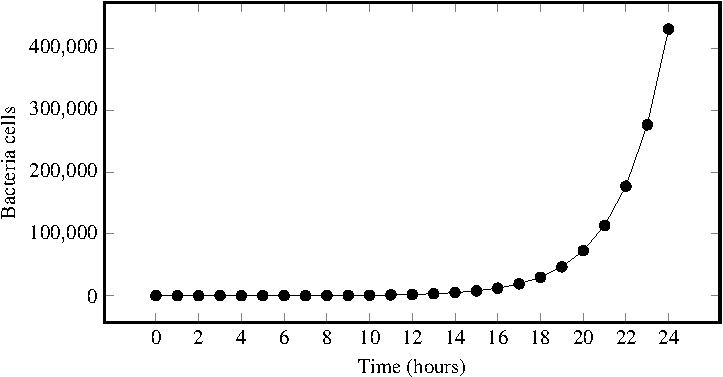
\includegraphics[scale=1.1]{image/11/bacteria.pdf}
\caption{%%
  The bacteria population in a Petri dish within $24$ hours.
  Initially, the Petri dish had a population of $10$ bacteria cells
  and the bacteria population is assumed to grow at a constant
  percentage rate of $56\%$ per hour.
}
\label{fig:bacteria_population_24_hours}
\end{figure}


%%%%%%%%%%%%%%%%%%%%%%%%%%%%%%%%%%%%%%%%%%%%%%%%%%%%%%%%%%%%%%%%%%%%%%%%%%%

\section{Exponential and linear growths}


%%%%%%%%%%%%%%%%%%%%%%%%%%%%%%%%%%%%%%%%%%%%%%%%%%%%%%%%%%%%%%%%%%%%%%%%%%%

\section{Compound interest}


%%%%%%%%%%%%%%%%%%%%%%%%%%%%%%%%%%%%%%%%%%%%%%%%%%%%%%%%%%%%%%%%%%%%%%%%%%%

\section{The number $e$}

\end{document}
